\documentclass{amsbook}
\usepackage{graphicx} % Required for inserting images
\usepackage{float}
\usepackage{hyperref}
\usepackage{amssymb}
\usepackage{mathtools}
\usepackage{tikz}
\usepackage[answerdelayed]{exercise}

\setlength{\parindent}{0pt}
\renewcommand{\ExerciseHeaderTitle}{\quad\ExerciseTitle}
\renewcommand{\AnswerHeader}{\medskip\centerline{\textbf{\ExerciseName\ \ExerciseHeaderNB}\smallskip}}
\renewcommand{\ExerciseHeader}{\ExerciseHeaderDifficulty{\textbf{\large \ExerciseName\ \ExerciseHeaderNB\ExerciseHeaderTitle \ExerciseHeaderOrigin\medskip}}}

\begin{document}

\title{Counting \& Probability:\\
    \Large Form V}

\author{M. Martynovsky}
\author{S. Chu}

\maketitle
\tableofcontents

\chapter{Sets}
\section{Set Notation}

\chapter{Combinatorics}
The section on counting and probability usually follows the unit on sequences and series. 
\section{Counting: Multiplication Principle A}
\begin{enumerate}
    \item 
\end{enumerate}
\section{Counting: Multiplication Principle B}

\section{Counting: Multiplication Principle C}

\section{Counting: Multiplication Principle D}

\section{Combinations A}

\vspace{.5cm}
\begin{figure}[H]
    \centering
    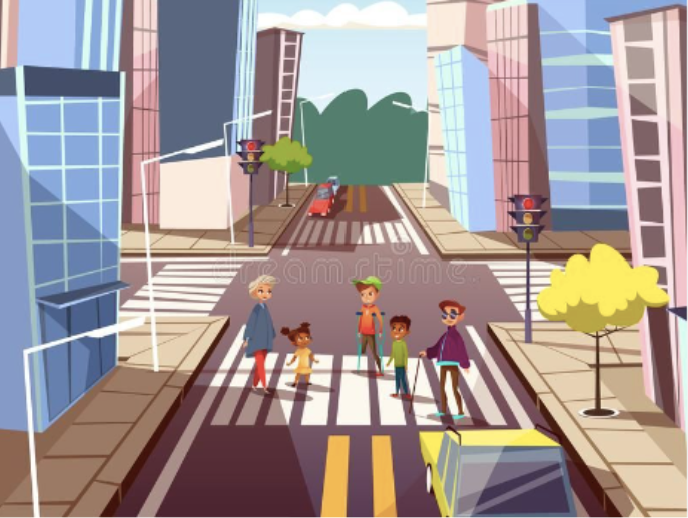
\includegraphics[scale=.5]{a.png}  
\end{figure}

\begin{Exercise}[title={Paths on a Grid},difficulty=1, label=c1]
The grid below represents the streets of a city. You are traveling from point $X$ to point $Y$ by moving either to the right or down. How may different routes are there from $X$ to $Y$? \refAnswer{\ExerciseLabel}
\begin{figure}[H]
    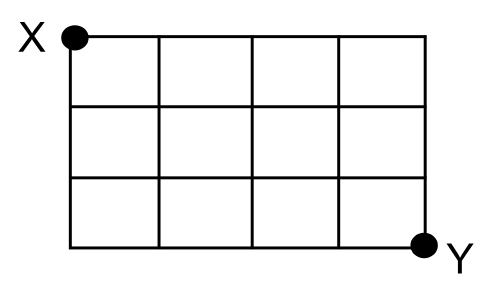
\includegraphics[scale=.5]{b.png}
\end{figure}
\end{Exercise}

\begin{Answer}[ref={c1}]
    There are 35 paths. You can arrive at this answer by recognizing each path 7 parts, 4 of which are to the right and 3 of which are down. You can count this either as $7 \choose 4$, choosing which 4 parts will be to the right, $7 \choose 3$, choosing which 3 parts will be down or $\frac{7!}{4!\cdot 3!}$ where you count the rearrangements of all 7 parts dividing out by repetitions.
\end{Answer}

\begin{Exercise}[title={Paths on a Grid II}, difficulty=2, label=c2]
Again the grid below represents the streets of a city. You are still traveling from $X$ to $Y$, but this time you must avoid passing through point $A$. How many routes are there from $X$ to $Y$ that do not pass through $A$? \refAnswer{\ExerciseLabel}
\begin{figure}[H]
    \centering
    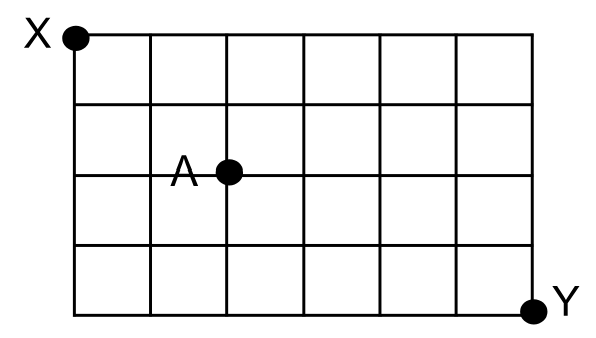
\includegraphics[scale=.55]{c.png}
\end{figure}
\end{Exercise}

\begin{Answer}[ref={c2}]
There are 120 paths. In this problem we want to avoid the point $A$. So we can first tally all the routes from $X$ to $Y$ as $10 \choose 6$, and then we take away all the paths that pass through $A$. There are two pieces to this journey. The trip from $X$ to $A$ can be done ${4 \choose 2} = 6$ ways, and the trip from $A$ to $Y$ can be done in ${6 \choose 2} =15$ ways. Using the multiplication counting principle this means there are $6\cdot 15 =90$ ways to go from $X$ to $Y$, passing through $A$. If we want to avoid point $A$ that means we will only have $210-90=120$ paths.
\end{Answer}



\chapter{Probability}


\chapter{Answers}
\shipoutAnswer

\end{document}
